%%%%%%%%%%%%%%%%%%%%%%%%%%%%%%%%%%%%%%%%%
% McMaster Masters/Doctoral Thesis
% LaTeX Template
% Version 2.2 (11/23/15)
%
% This template has been downloaded from:
% http://www.LaTeXTemplates.com
% Then subsequently from http://www.overleaf.com
%
% Version 2.0 major modifications by:
% Vel (vel@latextemplates.com)
%
% Original authors:
% Steven Gunn  (http://users.ecs.soton.ac.uk/srg/softwaretools/document/templates/)
% Sunil Patel (http://www.sunilpatel.co.uk/thesis-template/)
%
% Modified to McMaster format by Benjamin Furman (contact: https://www.xenben/com; Most up
% to date template at https://github.com/benjaminfurman/McMaster_Thesis_Template,
% occasionally updated on Overleaf template page)
%
% Modified for macdown by Antonio Paez; most up to date version at https://github.com/paezha/macdown
%
% License:
% CC BY-NC-SA 3.0 (http://creativecommons.org/licenses/by-nc-sa/3.0/)
%
%%%%%%%%%%%%%%%%%%%%%%%%%%%%%%%%%%%%%%%%%

%----------------------------------------------------------------------------------------
% DOCUMENT CONFIGURATIONS
%----------------------------------------------------------------------------------------

\documentclass[
11pt, % The default document font size, options: 10pt, 11pt, 12pt
oneside, % Two side (alternating margins) for binding by default, uncomment to switch to one side
english, % other languages available
singlespacing, % Single line spacing, alternatives: onehalfspacing or doublespacing
%draft, % Uncomment to enable draft mode (no pictures, no links, overfull hboxes indicated)
%nolistspacing, % If the document is onehalfspacing or doublespacing, uncomment this to set spacing in lists to single
%liststotoc, % Uncomment to add the list of figures/tables/etc to the table of contents
%toctotoc, % Uncomment to add the main table of contents to the table of contents
]{macthesis} % The class file specifying the document structure

%----------------------------------------------------------------------------------------
% Import packages here
%----------------------------------------------------------------------------------------
\usepackage[utf8]{inputenc} % Required for inputting international characters
\usepackage[T1]{fontenc} % Output font encoding for international characters
\usepackage{lastpage} % count pages
\usepackage{lmodern} % could change font type by calling a different package
\usepackage{lscape} % for landscaping pages
% New commands for landscape orientation
\newcommand{\blandscape}{\begin{landscape}}
\newcommand{\elandscape}{\end{landscape}}
%
\usepackage{siunitx} % for scientific units (micro-liter, etc)
\setcounter{tocdepth}{2} % so that only section and sub sections appear in Table of Contents. Remove or set depth to 3 to include sub-sub-sections

%----------------------------------------------------------------------------------------
% Define a blank page
%----------------------------------------------------------------------------------------
\def\blankpage{%
      \clearpage%
      \thispagestyle{empty}%
      \addtocounter{page}{-1}%
      \null%
      \clearpage}

%----------------------------------------------------------------------------------------
% Define a tight list
%----------------------------------------------------------------------------------------
\def\tightlist{}

%----------------------------------------------------------------------------------------
%	Highlight Code Chunks
%----------------------------------------------------------------------------------------
  \usepackage{color}
  \usepackage{fancyvrb}
  \newcommand{\VerbBar}{|}
  \newcommand{\VERB}{\Verb[commandchars=\\\{\}]}
  \DefineVerbatimEnvironment{Highlighting}{Verbatim}{commandchars=\\\{\}}
  % Add ',fontsize=\small' for more characters per line
  \usepackage{framed}
  \definecolor{shadecolor}{RGB}{248,248,248}
  \newenvironment{Shaded}{\begin{snugshade}}{\end{snugshade}}
  \newcommand{\AlertTok}[1]{\textcolor[rgb]{0.94,0.16,0.16}{#1}}
  \newcommand{\AnnotationTok}[1]{\textcolor[rgb]{0.56,0.35,0.01}{\textbf{\textit{#1}}}}
  \newcommand{\AttributeTok}[1]{\textcolor[rgb]{0.13,0.29,0.53}{#1}}
  \newcommand{\BaseNTok}[1]{\textcolor[rgb]{0.00,0.00,0.81}{#1}}
  \newcommand{\BuiltInTok}[1]{#1}
  \newcommand{\CharTok}[1]{\textcolor[rgb]{0.31,0.60,0.02}{#1}}
  \newcommand{\CommentTok}[1]{\textcolor[rgb]{0.56,0.35,0.01}{\textit{#1}}}
  \newcommand{\CommentVarTok}[1]{\textcolor[rgb]{0.56,0.35,0.01}{\textbf{\textit{#1}}}}
  \newcommand{\ConstantTok}[1]{\textcolor[rgb]{0.56,0.35,0.01}{#1}}
  \newcommand{\ControlFlowTok}[1]{\textcolor[rgb]{0.13,0.29,0.53}{\textbf{#1}}}
  \newcommand{\DataTypeTok}[1]{\textcolor[rgb]{0.13,0.29,0.53}{#1}}
  \newcommand{\DecValTok}[1]{\textcolor[rgb]{0.00,0.00,0.81}{#1}}
  \newcommand{\DocumentationTok}[1]{\textcolor[rgb]{0.56,0.35,0.01}{\textbf{\textit{#1}}}}
  \newcommand{\ErrorTok}[1]{\textcolor[rgb]{0.64,0.00,0.00}{\textbf{#1}}}
  \newcommand{\ExtensionTok}[1]{#1}
  \newcommand{\FloatTok}[1]{\textcolor[rgb]{0.00,0.00,0.81}{#1}}
  \newcommand{\FunctionTok}[1]{\textcolor[rgb]{0.13,0.29,0.53}{\textbf{#1}}}
  \newcommand{\ImportTok}[1]{#1}
  \newcommand{\InformationTok}[1]{\textcolor[rgb]{0.56,0.35,0.01}{\textbf{\textit{#1}}}}
  \newcommand{\KeywordTok}[1]{\textcolor[rgb]{0.13,0.29,0.53}{\textbf{#1}}}
  \newcommand{\NormalTok}[1]{#1}
  \newcommand{\OperatorTok}[1]{\textcolor[rgb]{0.81,0.36,0.00}{\textbf{#1}}}
  \newcommand{\OtherTok}[1]{\textcolor[rgb]{0.56,0.35,0.01}{#1}}
  \newcommand{\PreprocessorTok}[1]{\textcolor[rgb]{0.56,0.35,0.01}{\textit{#1}}}
  \newcommand{\RegionMarkerTok}[1]{#1}
  \newcommand{\SpecialCharTok}[1]{\textcolor[rgb]{0.81,0.36,0.00}{\textbf{#1}}}
  \newcommand{\SpecialStringTok}[1]{\textcolor[rgb]{0.31,0.60,0.02}{#1}}
  \newcommand{\StringTok}[1]{\textcolor[rgb]{0.31,0.60,0.02}{#1}}
  \newcommand{\VariableTok}[1]{\textcolor[rgb]{0.00,0.00,0.00}{#1}}
  \newcommand{\VerbatimStringTok}[1]{\textcolor[rgb]{0.31,0.60,0.02}{#1}}
  \newcommand{\WarningTok}[1]{\textcolor[rgb]{0.56,0.35,0.01}{\textbf{\textit{#1}}}}

%----------------------------------------------------------------------------------------
% Handling Citations
%----------------------------------------------------------------------------------------

% definitions for citeproc citations
\NewDocumentCommand\citeproctext{}{}
\NewDocumentCommand\citeproc{mm}{%
\begingroup\def\citeproctext{#2}\cite{#1}\endgroup}
\makeatletter
% allow citations to break across lines
\let\@cite@ofmt\@firstofone
% avoid brackets around text for \cite:
\def\@biblabel#1{}
\def\@cite#1#2{{#1\if@tempswa , #2\fi}}
\makeatother
\newlength{\cslhangindent}
\setlength{\cslhangindent}{1.5em}
\newlength{\csllabelwidth}
\setlength{\csllabelwidth}{3em}
\newenvironment{CSLReferences}[2] % #1 hanging-indent, #2 entry-spacing
{\begin{list}{}{%
	\setlength{\itemindent}{0pt}
	\setlength{\leftmargin}{0pt}
	\setlength{\parsep}{0pt}
	% turn on hanging indent if param 1 is 1
	\ifodd #1
	\setlength{\leftmargin}{\cslhangindent}
	\setlength{\itemindent}{-1\cslhangindent}
	\fi
	% set entry spacing
	\setlength{\itemsep}{#2\baselineskip}}}
{\end{list}}
\usepackage{calc}
\newcommand{\CSLBlock}[1]{\hfill\break\parbox[t]{\linewidth}{\strut\ignorespaces#1\strut}}
\newcommand{\CSLLeftMargin}[1]{\parbox[t]{\csllabelwidth}{\strut#1\strut}}
\newcommand{\CSLRightInline}[1]{\parbox[t]{\linewidth - \csllabelwidth}{\strut#1\strut}}
\newcommand{\CSLIndent}[1]{\hspace{\cslhangindent}#1}


%----------------------------------------------------------------------------------------
% Collect all your header information from the chapters here, things like acronyms, custom commands, necessary packages, etc.
%----------------------------------------------------------------------------------------
\usepackage{parskip} %this will put spaces between paragraphs
\setlength{\parindent}{15pt} % this will create and indent on all but the first paragraph of each section.
% should maybe change to glossaries package
\usepackage{acro}
\DeclareAcronym{est}{
	short = EST,
	long  = expressed sequence tags
}

\DeclareAcronym{Xl}{
	short = \textit{X.~laevis},
	long  = \textit{Xenopus~laevis}
}
\DeclareAcronym{Xg}{
	short = \textit{X.~gilli},
	long  = \textit{Xenopus~gilli}
}

\usepackage{etoolbox}
\preto\chapter{\acresetall} % resets acronyms for each chapter

\usepackage{xspace} %helps spacing with custom commands.
\newcommand{\oddname}{{\sc SoME goOfY LonG ThiNg With an AwkWarD NAme}\xspace}


\usepackage{pgfplotstable} % a much better way to handle tables
\pgfplotsset{compat=1.12}

% \usepackage{float} % if you need to demand figure/table placement, then this will allow you to use [H], which demands a figure placement. Beware, making LaTeX do things it doesn't want may lead to oddities.


%%%%
% LINK COLORS
% You can control the link colors at the end of the McMasterThesis.cls file. There is also a true/false option there to turn off all link colors.
%%%%


%----------------------------------------------------------------------------------------
%	THESIS INFORMATION
%----------------------------------------------------------------------------------------

\title{GEOG712 Course Project - Assessing the influence of tourists' perceived travel environment and their travel behavior on travel satisfaction using structural equation models (SEM): a case of Qinghai-Tibet Plateau}
%\thesistitle{Thesis Title} % Your thesis title, print it elsewhere with \ttitle
\author{Haoran Xu}
%\author{John \textsc{Smith}} % Your name, print it elsewhere with \authorname
\bdegree{B.Sc.}
\mdegree{}
%Previous degrees % print it elsewhere with \bdeg and \mdeg
\date{}
% The month and year that you submit your FINAL draft TO THE LIBRARY (May or December)
\university{McMaster University}
%\university{\href{http://www.mcmaster.ca/}{McMaster University}} % Your university's name and URL, print it elsewhere with \univname
%\division{}
\faculty{Faculty of Science} % Your faculty's name and URL, print it elsewhere with \facname
\department{School of Earth, Environment and Society} % Your department's name and URL, print it elsewhere with \deptname
\subject{Geography} % Your subject area, print it elsewhere with \subjectname
%\group{\href{http://researchgroup.university.com}{Research Group Name}} % Your research group's name and URL, print it elsewhere with \groupname
\supervisor{}
%\supervisor{Dr. Jane \textsc{Smith}} % Your supervisor's name, print it elsewhere with \supname
\examiner{} % Your examiner's name, print it elsewhere with \examname
\degree{Doctor of Philosophy}
%\degree{Doctor of Philosophy} % Your degree name, print it elsewhere with \degreename
\addresses{} % Your address, print it elsewhere with \addressname
\keywords{} % Keywords for your thesis, print it elsewhere with \keywordnames


% this sets up hyperlinks
\hypersetup{pdftitle=\ttitle} % Set the PDF's title to your title
\hypersetup{pdfauthor=\authorname} % Set the PDF's author to your name
\hypersetup{pdfkeywords=\keywordnames} % Set the PDF's keywords to your keywords

\begin{document}
\sloppy

\frontmatter % Use roman page numbering style (i, ii, iii, iv...) for the pre-content pages

\pagestyle{plain} % Default to the plain heading style until the thesis style is called for the body content

%----------------------------------------------------------------------------------------
%	Half Title (lay title)
%----------------------------------------------------------------------------------------
%\begin{halftitle} % could not get this environment working
%\vspace*{\fill}
\vspace{6cm}
\begin{center}
\ttitle
\end{center}
%\vspace*{\fill}
\pagenumbering{gobble} % leave this here, McMaster doesn't want this page numbered
%\end{halftitle}
\clearpage

%----------------------------------------------------------------------------------------
%	TITLE PAGE
%----------------------------------------------------------------------------------------
\pagenumbering{gobble}
\begin{center}

\vfill
\textsc{\Large \ttitle} \\

\vfill
{By \authorname\, \bdeg }


 \vfill
{\large \textit{A Thesis Submitted to the School of Graduate Studies in the Partial Fulfillment of the Requirements for the Degree \degreename}}\\

\vfill
{\large \univname\, \copyright\, Copyright by \authorname\, \today}\\[4cm] % replace \today with the submission date

\end{center}
\blankpage
\clearpage

%----------------------------------------------------------------------------------------
%	QUOTATION PAGE
%----------------------------------------------------------------------------------------

\vspace*{0.2\textheight}

\noindent{\itshape Hope in 2025 you can code more, better, and with confidence.}\bigbreak

\hfill\textemdash Haoran

\blankpage
\clearpage

%%%%%%%%%%%%%%%%%%%%%%%%%%%
%%%%%%%%%%%%%%%%%%%%%%%%%%%
% optional page stuff
%----------------------------------------------------------------------------------------
% can do physical constraints and symbols pages, see the original thesis example on overleaf if you want to include them at https://www.overleaf.com/latex/templates/template-for-a-masters-slash-doctoral-thesis/mkzrzktcbzfl#.VlPeicorpE4
%----------------------------------------------------------------------------------------

%----------------------------------------------------------------------------------------
%	DEDICATION
%----------------------------------------------------------------------------------------


\blankpage
\clearpage


%----------------------------------------------------------------------------------------
%	Descriptive note numbered ii
%----------------------------------------------------------------------------------------
% Need to add below info
\newpage
\pagenumbering{roman} % leave to turn numbering back on
\setcounter{page}{2} % leave here to make this page numbered ii, a Grad School requirement

\noindent % stops indent on next line
\univname \\
\degreename\, (\the\year) \\
Hamilton, Ontario (\deptname) \\[1.5cm]
TITLE: \ttitle \\
AUTHOR: \authorname\,  %list previous degrees
(\univname)  \\
SUPERVISOR: \supname\, \\
NUMBER OF PAGES: \pageref{lastoffront}, \pageref{LastPage}  % put in iv and number

\clearpage

%----------------------------------------------------------------------------------------
%	Lay abstract number iii
%----------------------------------------------------------------------------------------
% not actually included in most theses, though requested by the GSA
% uncomment below lines if you want to include one
\section*{Lay Abstract}
  The lay abstract must be 150 words or less.
  Hi this is the lay abstract.

  It must explain the key goals and contributions of the thesis in lay terms that are accessible to the general public.
\blankpage
\clearpage


%----------------------------------------------------------------------------------------
%	ABSTRACT PAGE number iv
%----------------------------------------------------------------------------------------

\section*{\Huge Abstract}
\addchaptertocentry{\abstractname}
% Type your abstract here.
This paper is the final project work for course GEOG712. It ueses a
\blankpage
\clearpage

%----------------------------------------------------------------------------------------
%	ACKNOWLEDGEMENTS
%----------------------------------------------------------------------------------------

  \begin{acknowledgements}
  \addchaptertocentry{\acknowledgementname} % Add the acknowledgments to the table of contents
    I would like to thank Dr.~Huaxiong Jiang and my undergrad fellows in old days for helping me with research design and questionnaire distributing. I would also like to thank Dr.~Antonio Paez for teaching this course and guiding me throughout the whole semester to learn from scratch about R and Github. With limited coding experiences before, I had been exposed to a lot of new ideas and thoughts on doing research itself. Mostly importantly, I am glad that I got to have the chance to build my own coding space little by little through detailed instructions, and that I could have little more confidence in coding skills instead of anxiety and upset. Anyways, this course surely would shed a very important light in my subsequent years of pursuing a PhD and a possible academic career.
  \end{acknowledgements}
\blankpage
\clearpage

%----------------------------------------------------------------------------------------
%	LIST OF CONTENTS/FIGURES/TABLES PAGES
%----------------------------------------------------------------------------------------

\tableofcontents % Prints the main table of contents

\listoffigures % Prints the list of figures

\listoftables % Prints the list of tables

%----------------------------------------------------------------------------------------
%	ABBREVIATIONS
%----------------------------------------------------------------------------------------
% many theses don't use this section, as it will be declared at first use and again each chapter. Uncomment these four lines to activate if you want
%\clearpage
%\section*{\Huge Acronyms}
%\addchaptertocentry{Acronyms}
%\printacronyms[name] % name without an option stops the header

%----------------------------------------------------------------------------------------
%	DECLARATION PAGE
%----------------------------------------------------------------------------------------

\begin{declaration}
\addchaptertocentry{\authorshipname}

\noindent I, \authorname, declare that this thesis titled, \emph{\ttitle} and the work presented in it are my own. I confirm that:

I did most of the research.

Also the writting.

Sometimes I cried.

But mostly I had fun.

\end{declaration}


%----------------------------------------------------------------------------------------
% The following bit is just here to make sure we end up on a new page and get the total number of roman numeral
\label{lastoffront}
\clearpage
% make sure this command is on the last of your frontmatter pages, i.e. only this command, a \clearpage then \mainmatter
% should be fine without modification
%----------------------------------------------------------------------------------------

%----------------------------------------------------------------------------------------
%	THESIS MAIN BODY
%----------------------------------------------------------------------------------------

\mainmatter % here the regular arabic numbering starts
\pagestyle{thesis}
\chapter{This is the degree you are aiming for with this thesis}\label{this-is-the-degree-you-are-aiming-for-with-this-thesis}

Placeholder

\chapter{Introduction and Background}\label{rmd-basics}

\section{Introduction}\label{introduction}

Subjective well-being is the psychological assessment of people's lives, including their emotional response to incidents and cognitive perceptions on life quality (Diener, 2000). The shift of well-being assessment from merely evaluating objective elements (wealth etc.) to incorporating multiple subjective indicators of assessment occurs in recent times as previous methods fail to determine the quality of life (De Vos, 2019; McCabe \& Johnson, 2013).

The relationships of tourism and SWB has been an emerging interest for many scholars to dig into. There are firm evidence that indicates tourism generally contributes to social tourists' well-being (McCabe \& Johnson, 2013). Scholars often use two-step surveys to explore the effect outdoor travel has on well-being improvement. Whilst another line of research focuses on the intrinsic mechanisms of the relationship, probing into how possible factors of tourism like built environment and travel behavior affect trip satisfaction and its internal interaction effects (Carneiro \& Eusébio, 2019). While among the varied indicators of detecting respondents' SWB, satisfaction is an effective factor to represent people's perceived subjective feeling towards a either short or long activity{[}Chen2019{]}.

This study digs into the relationships between travel satisfaction and other factors such as travel modes, travel frequency, travel distance and tourists' perceived tourist attraction environment and road environment. The core research questions is: what kind of factors would greatly impact local and non-local tourists' travel behavior and their travel satisfaction on Qinghai-Tibet Plateau.

\chapter{Data \& Methodology}\label{rmd-basics}

\section{Study Area and Data Collection}\label{study-area-and-data-collection}

The study area, Qinghai-Tibet Plateau, or referred to as Tibetan Plateau, is situated in the western region of China and characterized by its high altitude averaging over 4,000 meters. Due to its low population density and an extremely alpine climate, it exhibits a unique set of travel behavioral patterns for local residents or outside tourists. Furthermore, in recent years, the plateau has witnessed rapid infrastructural development invested by Chinese government, and a significant surge in tourist influx (Gao \& Sun, 2021). Despite this growth, scholarly investigations into travel behaviors, satisfaction levels, and the broader implications of these developments on local and visiting populations remain scant.

The questionnaire-collecting process started both online and on-site in July of 2022. The online questionnaires were written on the cover page that only those who had ever been to Qinghai-Tibet Plateau were qualified to fill out them. Then followed by was the on-site questionnaire-distributing process along with the Second Tibetan Plateau Scientific Expedition and Research Program during late July to early August. To specifically target at tourists while considering the convenience of conducting investigation, we mainly chose four touristic sites to collect questionnaires along the expedition route. Eventually, we collected 729 on-site questionnaires, which were acquired mostly in four sites - Qinghai Province Museum in Xining City, Qinghai Lake Scenic Area, Dachaidan Emerald Lake Scenic Area, Mani Stone Mound Scenic Area in Yushu City (Figure \ref{fig:SampleLocations}). With a total number of 830 questionnaires, 16 were filtered out due to a lot of missing answers, leaving 814 eventually entering modeling phase, with an validity rate of 98.07\%.

\begin{figure}
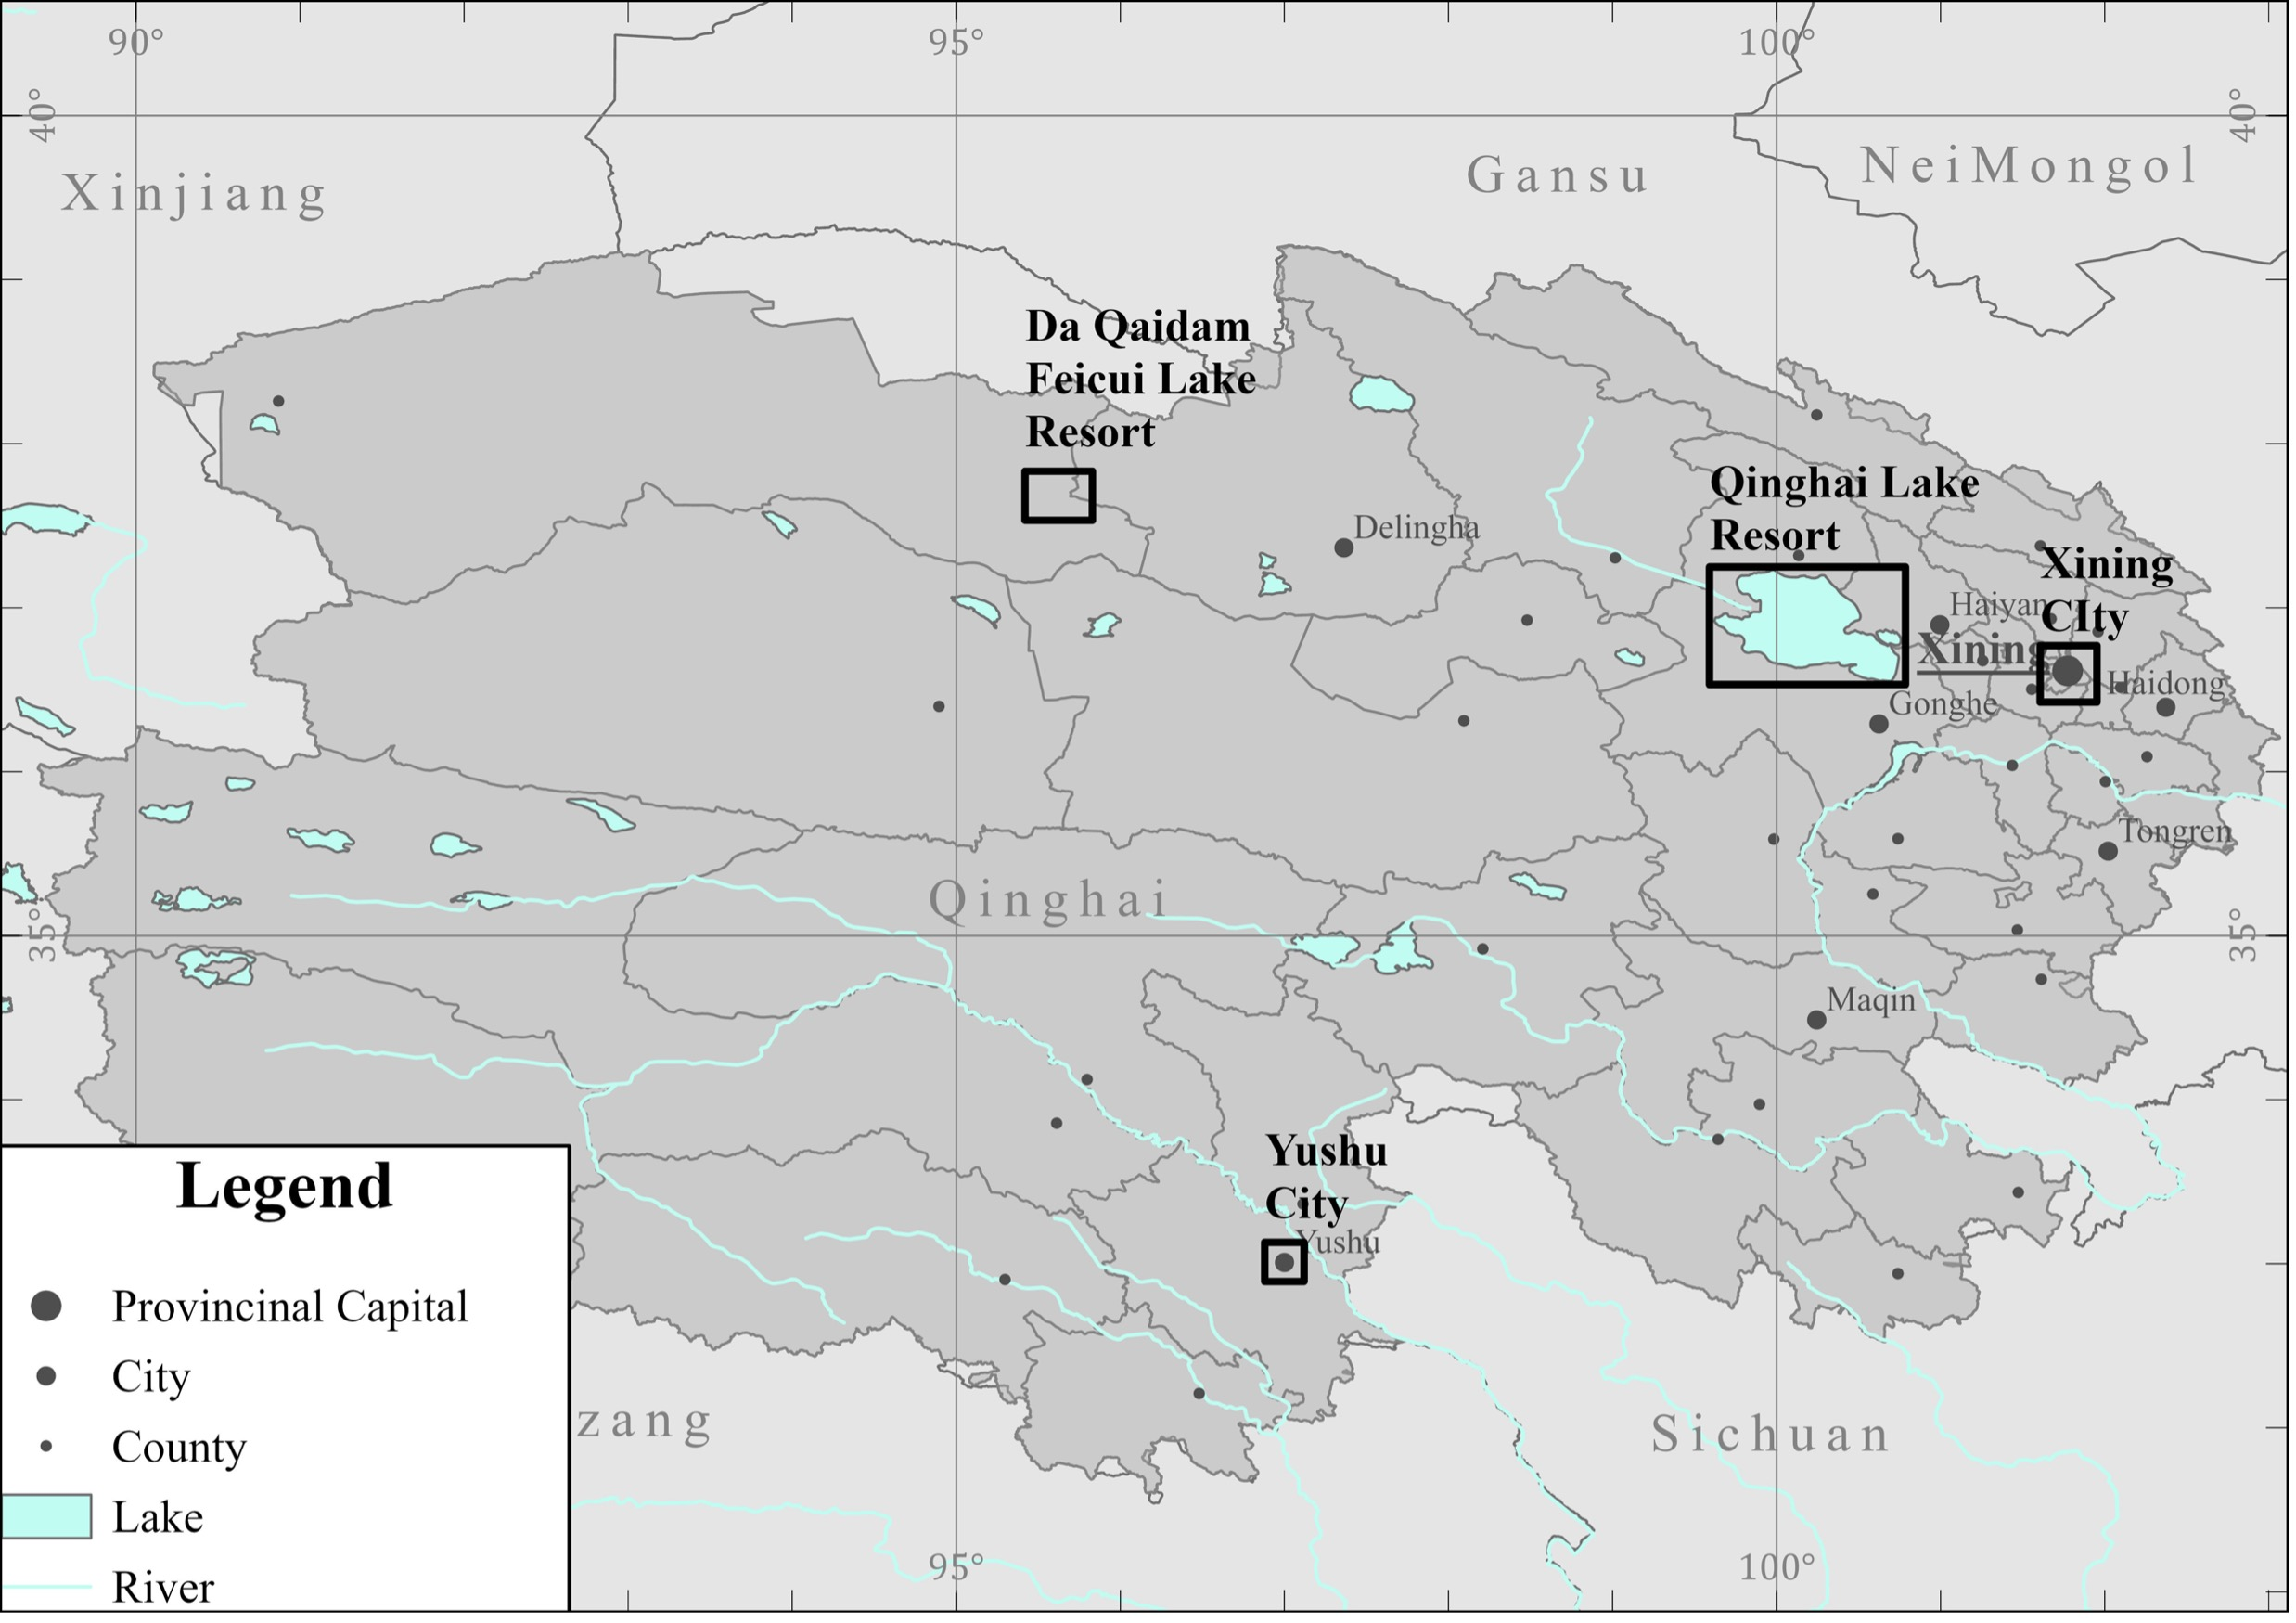
\includegraphics[width=0.8\linewidth]{figure/SampleLocations} \caption{\label{fig:SampleLocations}Sampling Locations on the Qinghai-Tibet Plateau}\label{fig:fig1-sample-locations}
\end{figure}

\section{Variables}\label{variables}

The survey was originally designed in the contexts of assessing smart transportation within the Qinghai-Tibet Plateau, which contains multifaceted aspects spanning from travel behavior, travel perceptions to technology adoption and usage. This study focuses only on several key dimensions, which are tourist travel behavior, their perceived travel environment, travel satisfaction, and their socio-demograpical characteristics.

The complete questionnaire (originally in Chinese and translated in English) alongside with data cleaning and re-digitalizing is stored in \texttt{TravelBehaviorQinghaiData} \href{https://github.com/Horan517/TravelBehaviorQinghaiData}{package}.

Specifically, socio-demograpical variables include gender, age, residence, personal monthly income, education level, profession, household size and ownership of driving license. Travel behavior variables in this model include frequency of traveling to Qinghai-Tibet Plateau in the past year and average daily traveling distance during the trip people were having when filling the questionnaire. Travel expectation and travel satisfaction are also measured, using a 5-point Likert scale ranging from strongly agree (value = 5) to strongly disagree (value = 1). Lastly, travel environment variables include two latent variables - people's perceptions of the environment of tourist attractions and the environment of roads along the trip, with the first consisting of 6 questions and the latter consisting of 5 questions.

\section{Methodology}\label{methodology}

Structural Equation Model (SEM) was used in the study to entangle the complex relationships across different variables. According to Bollen (1989), SEM is able to simultaneously estimate the causal relationships among a set of observed variables based on a specified model. In addition, SEM can calculate the indirect effects between two variables, mediated by other intervening variables (Hayes, 2009), which would help unravel the mediating effects of perceived travel environment had on travel satisfaction through travel behavior.

\section{Model Construction}\label{model-construction}

The conceptual framework of SEM model is shown in \ref{fig:}. Both direct and indirect pathways are drawn and measured, but only one model - a single-group model consisting of all observations, is measured in this model paper. A multi-group modelling approach (setting residence as a grouping variable) was previously used to compare the differences between local tourists and non-local tourists in the project. But in this model paper due to time constraints I did not incoporate the multi-group modelling analysis.

\begin{figure}
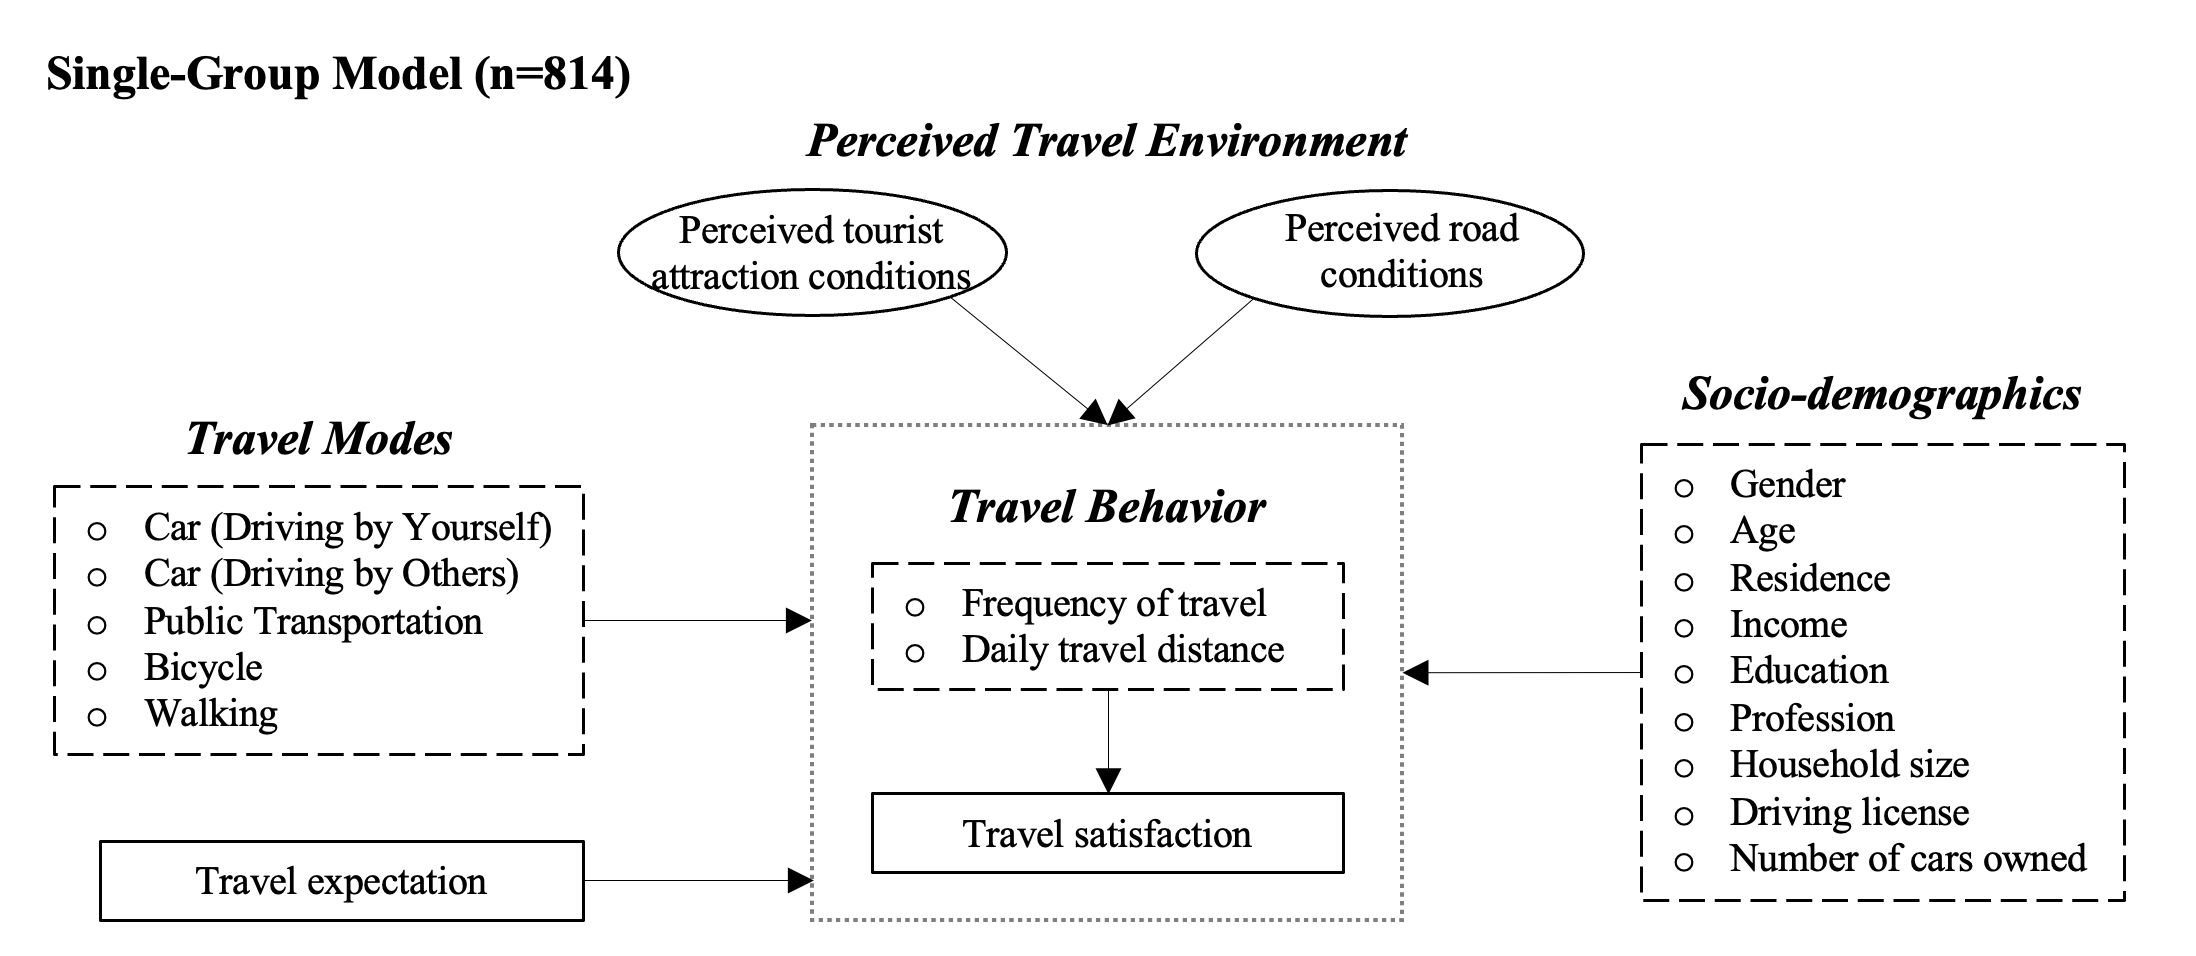
\includegraphics[width=0.8\linewidth]{figure/conceptual_framework} \caption{\label{fig:conceptual_framework} Conceptual Framework}\label{fig:fig2-conceptual-frmework}
\end{figure}

\section{Modeling}\label{modeling}

Below, confirmatory Factor Analysis (CFA) model and Structural Equation Modeling (SEM) model are respectively defined and measured.

\begin{Shaded}
\begin{Highlighting}[]
\CommentTok{\# Define the CFA model}
\NormalTok{cfa\_model }\OtherTok{\textless{}{-}} \StringTok{\textquotesingle{}}
\StringTok{\# Measurement model}
\StringTok{tourist\_envi =\textasciitilde{} ta\_envi1 + ta\_envi2 + ta\_envi3 + ta\_envi4 + ta\_envi5 + ta\_envi6}
\StringTok{road\_envi =\textasciitilde{} r\_envi1 + r\_envi2 + r\_envi3 + r\_envi4 + r\_envi5}
\StringTok{\textquotesingle{}}

\CommentTok{\# Fit the model}
\NormalTok{fit\_cfa }\OtherTok{\textless{}{-}} \FunctionTok{cfa}\NormalTok{(cfa\_model, }\AttributeTok{data =}\NormalTok{ TBQT, }\AttributeTok{missing =} \StringTok{"ml"}\NormalTok{)}

\CommentTok{\# Model summary}
\NormalTok{cfa\_summary }\OtherTok{\textless{}{-}} \FunctionTok{summary}\NormalTok{(fit\_cfa, }\AttributeTok{fit.measures =} \ConstantTok{TRUE}\NormalTok{)}
\end{Highlighting}
\end{Shaded}

\begin{Shaded}
\begin{Highlighting}[]
\CommentTok{\# Define the SEM model}
\NormalTok{model }\OtherTok{\textless{}{-}} \StringTok{\textquotesingle{}}
\StringTok{\# Measurement model}
\StringTok{tourist\_envi =\textasciitilde{} ta\_envi1 + ta\_envi2 + ta\_envi3 + ta\_envi4 + ta\_envi5 + ta\_envi6}
\StringTok{road\_envi =\textasciitilde{} r\_envi1 + r\_envi2 + r\_envi3 + r\_envi4 + r\_envi5}

\StringTok{\# Structural model}
\StringTok{frequency\_travel \textasciitilde{} gender + age + residence + income + edu\_lvl + profession + household\_size + dri\_lic + num\_cars + exp\_lvl + self\_drive + other\_drive + pub\_trans + bicycle + walking + tourist\_envi + road\_envi}
\StringTok{daily\_d \textasciitilde{} gender + age + residence + income + edu\_lvl + profession + household\_size + dri\_lic + num\_cars + exp\_lvl + self\_drive + other\_drive + pub\_trans + bicycle + walking + tourist\_envi + road\_envi}

\StringTok{sati\_lvl \textasciitilde{} gender + age + residence + income + edu\_lvl + profession + household\_size + dri\_lic + num\_cars + exp\_lvl + self\_drive + other\_drive + pub\_trans + bicycle + walking + tourist\_envi + road\_envi}
\StringTok{sati\_lvl \textasciitilde{} frequency\_travel + daily\_d}

\StringTok{\# Correlations}
\StringTok{r\_envi1 \textasciitilde{}\textasciitilde{} r\_envi2}
\StringTok{exp\_lvl \textasciitilde{}\textasciitilde{} tourist\_envi}
\StringTok{ta\_envi1 \textasciitilde{}\textasciitilde{} ta\_envi2}
\StringTok{ta\_envi5 \textasciitilde{}\textasciitilde{} ta\_envi6}
\StringTok{\textquotesingle{}}

\CommentTok{\# Fit the model}
\NormalTok{fit\_sem }\OtherTok{\textless{}{-}} \FunctionTok{sem}\NormalTok{(model, }\AttributeTok{data =}\NormalTok{ TBQT, }\AttributeTok{estimator =} \StringTok{"MLR"}\NormalTok{, }\AttributeTok{std.lv =} \ConstantTok{TRUE}\NormalTok{, }\AttributeTok{missing =} \StringTok{"ml"}\NormalTok{)}
\CommentTok{\# case{-}wise (or ‘full information’) maximum likelihood estimation (setting \textasciigrave{}\textasciigrave{}) cannot be used if using "WLSMV" to treat the problem of categorical endogenous variales.}

\CommentTok{\# Model summary}
\FunctionTok{fitMeasures}\NormalTok{(fit\_sem, }\FunctionTok{c}\NormalTok{(}\StringTok{"rmsea"}\NormalTok{, }\StringTok{"cfi"}\NormalTok{, }\StringTok{"tli"}\NormalTok{, }\StringTok{"chisq"}\NormalTok{, }\StringTok{"df"}\NormalTok{))}
\NormalTok{sem\_summary }\OtherTok{\textless{}{-}} \FunctionTok{summary}\NormalTok{(fit\_sem, }\AttributeTok{fit.measures =} \ConstantTok{TRUE}\NormalTok{, }\AttributeTok{standardized =} \ConstantTok{TRUE}\NormalTok{, }\AttributeTok{modindices =} \ConstantTok{TRUE}\NormalTok{)}

\NormalTok{mi }\OtherTok{\textless{}{-}} \FunctionTok{modindices}\NormalTok{(fit\_sem, }\AttributeTok{sort =} \ConstantTok{TRUE}\NormalTok{, }\AttributeTok{maximum.number =} \DecValTok{20}\NormalTok{)}
\end{Highlighting}
\end{Shaded}

As all of the variables in the model are categorical variables (either binary, categorical or ordinal), \texttt{lavaan} package only need to maintain the types of these categorical variables as \texttt{numeric} to deal with exogenous categorical variables. For endogenous variables, the ideal way is to set it as \texttt{ordered}, however, since the Full Information Maximum Likelihood method of dealing with missing value cannot deal with categorical variable. Therefore, I prioritized using Maximum Likelihood with Robust Standard Errors (MLR) estimator with setting \texttt{missing\ =\ "ml"} to deal with missing values.

For iterations, as the iterations control is already built into the \texttt{lavaan} package, it will automatically iterate until convergence. Regarding bootstrapping strategy, it helps to deal with data non-normality problem and to test indirect effects by estimating bias-corrected confidence intervals (CI). This method should be tested with trials, yet due to time constraints, it is not included in this model paper.

\chapter{Results}\label{rmd-basics}

Placeholder

\section{Statistical Results}\label{statistical-results}

\section{CFA Results}\label{cfa-results}

\section{SEM Results}\label{sem-results}

\chapter*{Conclusion}\label{conclusion}
\addcontentsline{toc}{chapter}{Conclusion}

If we don't want Conclusion to have a chapter number next to it, we can add the \texttt{\{-\}} attribute.

\textbf{More info}

And here's some other random info: the first paragraph after a chapter title or section head \emph{shouldn't be} indented, because indents are to tell the reader that you're starting a new paragraph. Since that's obvious after a chapter or section title, proper typesetting doesn't add an indent there.

\chapter*{References}\label{references}
\addcontentsline{toc}{chapter}{References}

Placeholder

\chapter{TBQTSEM}\label{tbqtsem}

Placeholder

\phantomsection\label{refs}
\begin{CSLReferences}{1}{0}
\bibitem[\citeproctext]{ref-Bollen1989}
Bollen, K. A. (1989). Structural equation models with observed variables. In \emph{Structural equations with latent variables} (pp. 80--150). John Wiley \& Sons, Ltd. http://doi.org/\href{https://doi.org/10.1002/9781118619179.ch4}{10.1002/9781118619179.ch4}

\bibitem[\citeproctext]{ref-Carneiro2019}
Carneiro, M. J., \& Eusébio, C. (2019). Factors influencing the impact of tourism on happiness. \emph{Anatolia}, \emph{30}(4), 475--496. http://doi.org/\href{https://doi.org/10.1080/13032917.2019.1632909}{10.1080/13032917.2019.1632909}

\bibitem[\citeproctext]{ref-DeVos2019}
De Vos, J. (2019). Analysing the effect of trip satisfaction on satisfaction with the leisure activity at the destination of the trip, in relationship with life satisfaction. \emph{Transportation}, \emph{46}, 623--645. http://doi.org/\href{https://doi.org/10.1007/s11116-017-9812-0}{10.1007/s11116-017-9812-0}

\bibitem[\citeproctext]{ref-Diener2000}
Diener, E. (2000). Subjective well-being: The science of happiness and a proposal for a national index. \emph{American Psychologist}, \emph{55}(1), 34--43.

\bibitem[\citeproctext]{ref-Gao2021}
Gao, X., \& Sun, D. (2021). Transport accessibility and social demand: A case study of the tibetan plateau. \emph{PLOS ONE}, \emph{16}(9), e0257028. http://doi.org/\href{https://doi.org/10.1371/journal.pone.0257028}{10.1371/journal.pone.0257028}

\bibitem[\citeproctext]{ref-Hayes2009}
Hayes, A. F. (2009). Beyond baron and kenny: Statistical mediation analysis in the new millennium. \emph{Communication Monographs}, \emph{76}(4), 408--420. http://doi.org/\href{https://doi.org/10.1080/03637750903310360}{10.1080/03637750903310360}

\bibitem[\citeproctext]{ref-McCabe2013}
McCabe, S., \& Johnson, S. (2013). The happiness factor in tourism: Subjective well-being and social tourism. \emph{Annals of Tourism Research}, \emph{41}, 42--65. http://doi.org/\href{https://doi.org/10.1016/j.annals.2012.12.001}{10.1016/j.annals.2012.12.001}

\end{CSLReferences}

\end{document}
